\documentclass[10pt]{book} 
\usepackage[letterpaper, portrait, margin=0.5in]{geometry} 
\usepackage{pbsi}

\usepackage{sectsty}
\sectionfont{\Huge}
\subsectionfont{\LARGE}
\subsubsectionfont{\Large}

\usepackage{float}
\usepackage{graphicx}
\usepackage{subfig}


\usepackage{hyperref}
\hypersetup{colorlinks=true, linkcolor=blue, filecolor=magenta, urlcolor=cyan}

\usepackage{amsmath}

\usepackage[framemethod=TikZ]{mdframed}
\usepackage{listings}
\usepackage{courier}
\definecolor{backgroundgray}{RGB}{40, 40, 40}
\definecolor{backgrounddarkgray}{RGB}{10, 10, 10} % for terminal
\definecolor{black}{rgb}{1,1,1} % border around code; dont edit this
\definecolor{white}{rgb}{1,1,1} % border around code
\definecolor{textgray}{rgb}{0.98,0.98,0.98} % basic text
\definecolor{commentgray}{rgb}{0.5,0.5,0.5} % basic text
\definecolor{stringgreen}{rgb}{0.596,0.592,0.102} % string
\definecolor{myred}{rgb}{0.9,0.2,0.2} % string
\definecolor{keywordorange}{rgb}{0.9,0.5,0} % keywords
\definecolor{mypurple}{rgb}{1.0,0.2,0.2} % headers

\lstset{frame=tb,
  language=c++,
  basicstyle={\small\ttfamily},
  breakatwhitespace=false,       
  breaklines=true,               
  commentstyle=\color{dkgreen},   
  deletekeywords={...},          
  escapeinside={\%*}{*)},                  
  frame=single,                  
  morekeywords={BRIEFDescriptorConfig,string,TiXmlNode,DetectorDescriptorConfigContainer,istringstream,cerr,exit}, 
  identifierstyle=\color{white},
  stringstyle=\color{stringgreen},
  numberstyle=\tiny\color{textgray},
  directivestyle=\color{myred},
  tabsize=4,                     
  aboveskip=3mm,
  belowskip=3mm,
  showstringspaces=false,
  columns=flexible,
  numbers=none,
  commentstyle=\itshape\color{commentgray},
  emph={int,char,double,float,unsigned},
  emphstyle={\color{orange}},
  keywordstyle=\color{keywordorange},
  frame=single,	                   % adds a frame around the code
  escapeinside={<@}{@>},
  keepspaces=true,
  breaklines=true,
  breakatwhitespace=true,
}


\begin{document} 
\title{\Huge \bsifamily Notes on OpenCL}
\author{\textit{by Ramkumar Narayanan}}
\date{}
\maketitle 
\tableofcontents
\newpage

% ----------------------------------------------------------------------------------------------------------------
{\color{red} \date{30-May-2020}}
\Large
\chapter{Introduction to OpenCL}
\section{What is OpenCL?}
OpenCL is an industry standard for programming devices composed of a combination of CPU's, GPU's and other processors. This platform enables heterogeneous, distributed computing. OpenCL exposes the hardware. It does not attempt to hide it behind its abstractions. From a hardware perspective, we are tending towards obtaining maximum compute power per watt expenditure. 

Parallel hardware needs parallel software. This can be introduced with the concept of concurrency. Concurrency means running more than one stream of operations. Challenge is to find points of concurrency in a software system and express it as a source code. The resulting concurrent programs should deliver performance. Finding concurrency is pretty challengingand sometimes tricky. Coding up concurrency is the crus of the problem. Abstraction is often required to make the prallel program more manageable. 

\section{Programming Models}
This is a very high level description of the heteregeneous system. Basically there are two broad types of parallelism 1) \textit{\textbf{task parallelism}} and \textit{\textbf{data parallelism}}. Programmers break the problem down to individual tasks and then focus on how to bring about concurrency. This is easiest when tasks are independent. However, even when data is shared, this can be achieved. Concepts like load balancing comes here.

\begin{figure}[H]
  \centering
  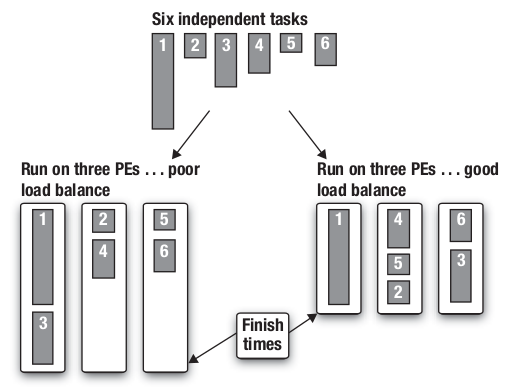
\includegraphics[scale=0.5]{./images/load_balancing.png}
  \caption{Load balancing of different tasks}
  \label{load balancing}
\end{figure}

In \textit{\textbf{data parallelism}} programmers update chunks of data elements in parallel. programmers think of their problems in terms of data elements.

\begin{figure}[H]
  \centering
  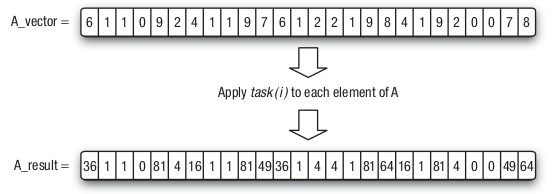
\includegraphics[scale=0.7]{./images/data_parallelism.png}
  \caption{Data parallelism where a single task is applied concurrently to many data elements}
  \label{data parallelism}
\end{figure}

\subsection{Platform Model}
\begin{enumerate}
	\item \textbf{\textit{Host:}} A device that controls all the OpenCL compatible devices. This is where the main entry point of the program. The host itself could be an OpenCL compatible device.
	\item \textbf{\textit{Compute Devices:}} Each graphics card or the CPU or FPGA's form what is called the compute device. All the compute devies are visible by the host.
	\item \textbf{\textit{Compute Units}} Like the several cores of the processor whether it be a GPU or a CPU. 
	\item \textbf{\textit{Processing Elements:}} Each core will have several small units that does the actual processing call the processing elements.
\end{enumerate}

\begin{figure}[H]
  \centering
  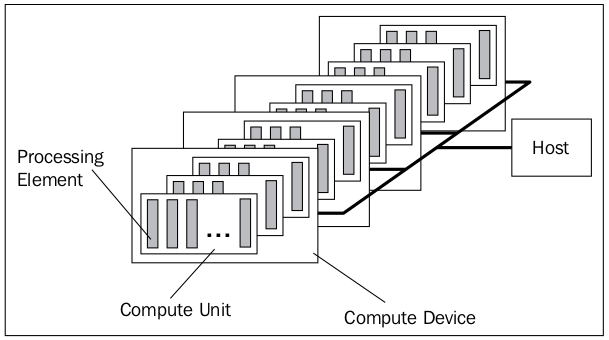
\includegraphics[scale=0.4]{./images/platform_model.png}
  \caption{OpenCL platform model}
  \label{platform_model}
\end{figure}

\subsection{Execution Model}
An OpenCL program has two distinct parts: 1) \textbf{\textit{Host}} program and 2) a collection of one or more \textbf{\textit{kernels}}. Host program runs on the host. Host program is our normal cpp or python code. OpenCL does not define how that is programmed - only how it interacts with the compute device(s).
\begin{enumerate}
	\item \textbf{\textit{OpenCL Kernels:}} Written in C language and compiled with the OpenCL C compiler.
	\item \textbf{\textit{Native Kernels:}} These functions are created outside OpenCL and accesssed within OpenCL through a function pointer.
\end{enumerate}

\textit{\textbf{How does a kernel execute on the OpenCL device?}} A kernel is defined on the host. The host program issues a command that submits the kernel for execution. When this command is issued, OpenCL runtime creates what is called the \textit{\textbf{index space}}. An instance of kernel executes for each point in the index space. Each instance of the executing kernel is called a \textit{\textbf{work item}}. A work item is identified by the coordinates in the index space. The behaviour of each kernel execution can differ due to branch statements in the execution. Work items are organized into work groups providing a more coarse grained decomposition of the index space. Work groups exactly span the index space. Work groups are of the same size. There are relative and global ID's for work groups and work items. Work items within a workgroup executes concurrently and workgroups may/may-not execute concurrently. The index space spans N-dimensions hence called the NDRange. Currently N can span 1, 2 or 3 dimensions. Let us take a look at the schemes using a 2D Range example.

\subsubsection{NDRange and associated notations}
Lets take a look at some definitions and some notations
\begin{enumerate}
	\item $G_x$ and $G_y$ - indicates the sizes of the index space.
	\item $W_x$ and $W_y$ - index space is chopped into so many work groups.
	\item $L_x$ and $L_y$ - individual work group size after chopping.
	\item $(g_x,g_y)$ - represents the global coordinates of the work item.
	\item $(w_x, w_y)$ - represents the coordinates of the work group.
	\item $(l_x,l_y)$ - represents work item coordinate within the work group.
\end{enumerate}

Take a look at the next image.

\begin{figure}[H]
  \centering
  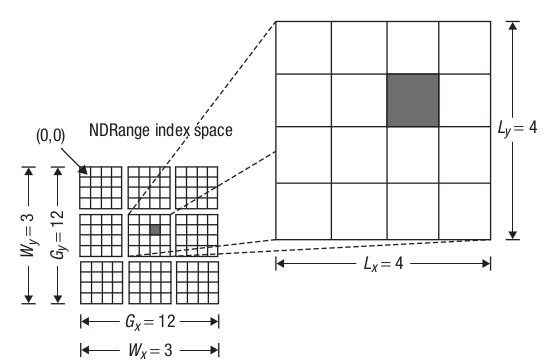
\includegraphics[scale=0.6]{./images/NDRange.png}
  \caption{NDrange, work group, work id}
  \label{}
\end{figure}

Number of work groups, $W_x=G_x/L_x$ and $W_y=G_y/L_y$.

\begin{enumerate}
	\item $(G_x,G_y)$ = $(12,12)$
	\item $(W_x,W_y)$ = $(3,3)$
	\item $(L_x,L_y)$ = $(4,4)$
	\item $(g_x,g_y)$ = $(6,5)$
	\item $(w_x,w_y)$ = $(1,1)$
	\item $(l_x,l_y)$ = $(2,1)$
\end{enumerate}

\subsubsection{Context} 
Computation of the kernels is always done on the OpenCL devices. However, the host has a very important job of setting up various stuff. For instance, the host defines the NDRange and the queues that control the details of how and when the kernels execute. All these definitions are contained in the API's within the OpenCL definition.

A context defines these environmental parameters within which the kernels are defined and executed. To be more precise, context is defined in the following terms,

\begin{enumerate}
	\item \textit{\textbf{Devices:}} A collection of OpenCL devices used by the host.
	\item \textit{\textbf{Kernels:}} A collection of OpenCL functions that run on the devices.
	\item \textit{\textbf{Program Objects:}} The source code and executables that implement kernels.
	\item \textit{\textbf{Memory Objects:}} a set of objects in memory that are visible to OpenCL devices and contain values that can be operated by instances of kernels. The host has a familiar memory description. However, OpenCL programs can run on several devices of different types. All the memory layout schemes will not be familiar to the host. To deal with this we need some sort of memory mapping defined by \textit{memory objects}.
\end{enumerate}
\vspace{1cm}
{\color{red} \date{01-June-2021}}
\subsubsection{Command Queues}
Now, let us take a look at how the host issues commands to OpenCL devices. The interaction between host and OpenCL devices happens through commands posted by the host on the command queue. These commands wait in the command queue until they are executed on an OpenCL device. A command queue is created by the host and attached to a single OpenCL device after the context has been defined. OpenCL supports three types of commands.
\begin{enumerate}
	\item \textit{\textbf{Kernel execution commands:}} executes a kernel on the processing elements of an OpenCL device.
	\item \textit{\textbf{Memory Commands:}} transfer data between host and different memory objects, move data between memory objects, or map and unmap memory objects from the host's address space.
	\item \textit{\textbf{Synchronization commands:}} put constraints on the order in which the commands executes.
\end{enumerate}

This is the \textit{\textbf{flow of control}} in a program $\rightarrow$ the programmer defines the context, command queues, memory and program objects. He/she also builds the data structures on the host to support the application. Then the focus shifts to the command queues. Memory objects are moved from the host onto the devices; kernel arguments are attached to memory objects and then submitted to command queues for execution. When a kernel has completd its work, memory objects produced in the computation is copied back to the host.

\textit{\textbf{Synchronization}} is required in many cases. One example would be, the kernels that execute later might have to wait for the completion of the previous kernel's execution to access the memory. Synchronization commands are used here.

The host submits the commands to the command queue and the device(s) proceed without waiting for the host to give any other command. The host then waits for the devices to finish execution and get back to the host. Within the command queue itself there are two schemes. \textit{\textbf{In-order execution}} commands are launched in the order they appear in the command queue. In other words the previous command execution is completed before the next one even begins. In \textit{\textbf{Out-of-order execution}} commands do not wait for the previous command to complete before the next on starts.

Out-of-order executions are used in automatic load balancing. Its a well known technique used in design of parallel algorithms driven by command queues (see the Master-Worker pattern in T.G. Mattson et al., Patterns for Parallel Programming). This can potentially lead to a disaster if not managed properly. Data by a kernel run can be accessed before its updated by the previous kernel. Sophisticated synchronization protocols in addition to simple synchronization commands are used. Commands submitted to command queues generate event objects. A command can be told to wait until certain condition on the event objects exist. These events can be used to coordinate execution between the host and the OpenCL devices. 

Also, multiple command queues can be associated with a single context. The queues run concurrently and independently with no explicit mechanisms within OpenCL to synchronize between them.

\subsection{Memory Model}
In memory model we will learn how host interacts with the devices in terms of data access. OpenCL defines two types of memory objects 1) \textit{\textbf{buffer objects}} and 2) \textit{\textbf{image objects}}. A \textit{\textbf{buffer object}} is a contiguous block of memory and a programmer can map data structures onto this buffer and access it through pointers. This provides flexibility to define about any data structure the programmer wishes. \textit{\textbf{Image objects}} on the other hand are restricted to holding images. The image memory object is an opaque object. OpenCL provides functions to manipulate images, but the contents of the image themselves are opaque to the kernel program. Subregions of a memory region can be made a separate memory object that can be manipulated through a command queue.
% TODO(ram): did not fully understand the above.

OpenCL defines 5 distinct memory regions
\begin{enumerate}
	\item \textit{\textbf{Host Memory:}} this memory region is only visible to the host.
	\item \textit{\textbf{Global Memory:}} This memory region permits read/write access to all work items and work groups. Read/writes can be cached depending on the capabilities of the device.
	\item \textit{\textbf{Constant Memory:}} This memory region of global memory remains constant during the execution of the kernal. Host allocates and initializes this memory. Work items have only read access to this.
	\item \textit{\textbf{Local Memory:}} This memory region is local to the work group. This memory region can allocated variables that are shared by all work items in the work group. Local memory can be mapped onto sections of the global memory.
	\item \textit{\textbf{Private Memory:}} This is a private region to the work item. Variables defined here are private and not visible to the other work items.
\end{enumerate}

\textit{\textbf{Work items}} run on \textit{\textbf{processing elements}} and have their own \textit{\textbf{private memory}}.

\textit{\textbf{Work Group}} runs on a \textit{\textbf{compute unit}} and shares a \textit{\textbf{local memory}} region with the work items in the work group. The OpenCL \textit{\textbf{OpenCL device memory}} works with the host to support the \textit{\textbf{global memory}}.

The host and OpenCL device memory models are for the most part independent of each other. The host is defined outside OpenCL. However, they do interact at times. This is through explicit memory transfer or by mapping and unmapping regions of memory objects. To copy data, host enqueues commands to transfer data between memory object and host memory. The memory transfer commands may be blocking or non-blocking. For a blocking memory transfer, the OpenCL function call returns once the associated memory resources on the host can be safely reused. For a non-blocking memory transfer, OpenCL function call returns as soon as the command is enqueued regardless of whether the host memory is safe to use.
 Mapping/un-mapping method of interaction between the host and the OpenCL memory objects allows the host to map a retion from the memory to its own address space. The \textit{\textbf{memory map}} command is enqueued in the command queue just like any other command. They can be blocking or non-blocking. Once a region from the memory object has been mapped, the host can read or write to this region. The host unmaps the region when access to this mapped region by the host is complete.

\begin{figure}[H]
  \centering
  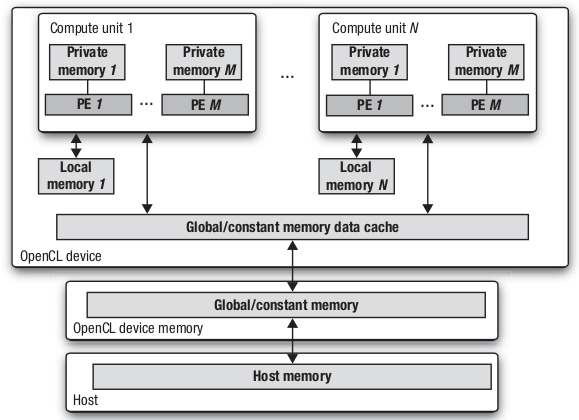
\includegraphics[scale=0.8]{./images/memory_mapping.png}
  \caption{Memory mapping}
	\label{}
\end{figure}

{\color{red} \date{02-June-2020}} \\
Let us start with \textit{private memory}. This is not visible to the host. It is visible only to an individual work item. The memory follows a load/store memory model familiar to sequential programming. \textit{Local Memory} has values seen by a set of work items. They have these things called barriers which are rules defined when the memory is accessible. In other words, a barrier marks a point in the execution of the set of work items where the memory is guaranteed to be cin a consistent and known state before the execution continues. For \textit{global memory}, barriers are also set at the work group level as there is no way to enforce consistency of global memory between the different work groups executing a kernel.

OpenCL also defines a \textit{\textbf{relaxed consistency}} model. The values seen in memory by an individual work-item where the load/store update rules are a bit relaxed.

Consistency of memory in OpenCL can be defined in many ways. For \textit{in-order execution}, all work items associated with the kernel complete execution and then memory can be modified. For \textit{out-of-order execution}, synchronization points can be setup or they can be explicitly managed through event mechanisms.

\subsection{Programming Models}
The previous model description was a \textit{hardware centric} model description. We now shift gears and describe how we map parallel algorithms onto OpenCL using a programming model. Programming models are intimately connected to how programmers reason about their algorithms. OpenCL programming models are defined with two programming models in mind 1) task parallelism, 2) data parallelism. Also, there is a hybrid model: tasks that contain data parallelism. We can see finer nuances of programming models that can be constructed overtime. Let us now look at the basic programming models.

\subsubsection{Data-Parallel Programming Model}
Concurrent kernel operations are carried out on homogeneous pieces of data simultaneously. All and any updates are concurrent. The key to this is in the NDRange. The programmer aligns the data to the defined NDRange perfectly to carry out the operations. In more complicated data-parallel problems, data is stored in the local memory and shared between all the work items of the work group. Note work group barriers are setup as synchronization points for controlling data load/store. All work items within a group should adhere to this barrier before proceeding. OpenCL however, does not describe any mechanisms for syncing between work groups. This is something which the programmer should keep in mind.

OpenCL provides a hierarchial model of data parallelism: data parallelism within a work-group and data parallelism between work-groups. OpenCL specification discusses two variants of this form of data parallelism. In the \textit{\textbf{explicit model}} the entire control of creating this is with the programmer. In the \textit{\textbf{implicit model}} the programmer just defines the NDRange and leaves the system to choose the work-groups.

\textit{\textbf{Single Instruction Multiple Data, SIMD}} is where there are no branch statements and each kernel execution operates on a piece of data dictated by its global ID. When there are branch statements, it is called \textit{\textbf{Single Program Multiple Data, SPMD}}. OpenCL supports both SIMD and SPMD. Obviously, SIMD is far more efficient.

%TODO(ram): Page 26 in the textbook about integration - visit it later on. 

\subsubsection{Task-Parallelism Programming Model}
The OpenCL execution model was clearly designed with data parallelism as a primary target. However it supports a rich array of task-parallelism algorithms also. We can see three types of paradigms in task parallel modelling
\begin{enumerate}
	\item When a single kernel is submitted in the command queue and the kernel operates over different data types for the same operation.
	\item The second version is when a queue of different tasks are submitted to the command queue for an out-of-order execution.
	\item lastly when a task graph is used along with OpenCL's event model.
\end{enumerate}
\subsection{OpenCL Frameworks - Contents of OpenCL}

\begin{enumerate}
	\item \textit{\textbf{OpenCL Platform API:}} The platform API defines function used by the host program to discover OpenCL devices an their capabilities as well as to create context for OpenCL applications.
	\item \textit{\textbf{OpenCL runtime API:}} This API manipulates the context to create command-queues and other operations that occur at runtime. Commands to submit to the command queue comes from here.
	\item \textit{\textbf{The OpenCL Programming Language:}} This is the language used by the kernels.
\end{enumerate}

\subsubsection{Platform API}
The term \textit{platform} has a specific meaning in OpenCL. Multiple OpenCL platforms can exist on a single heteregeneous system with a CPU and several GPUs. Each device vendor can provide an implementation for OpenCL. Which one to use with its query capabilities are dealt with by the platform API. 

\subsubsection{Runtime API}
The functions of the platform API defines the context for an OpenCL application. The runtime API focuses on using the defined context to service the needs of the applictaion. This is large and complex list of functions.

The first job is to define a command queue. One/multiple command queue can be attached to a single context. With command-queues in place, the runtime API is now used for memory management such as defining memory objects and manipulating them. Managing memory objects is an important task. Supporting garbage collection, retaining/releasing memory etc.

Runtime API also creates dynamic libraries from where kernels are defined. The program objects, the compiler to compile them and the definitions of all the kernels are handled by the runtime layer.

Commands that interact with the command-queue, synchronization points etc are all handled by the runtime layer. This does most of the heavy lifiting.

\subsubsection{Kernel Programming Language}
This are similar to shaders in OpenGL and they do most of the work in the OpenCL application. The kernel programming langugae in OpenCL is called the OpenCL C programming language because its derived out of ISO C99 langugage. Some of the major fields deleted from this language constructs include

\begin{enumerate}
	\item Recursive functions
	\item Pointers to functions
	\item Bit fields
\end{enumerate}

\subsection{OpenCL Summary}
The OpenCL execution pipeline somewhat looks like the below image

\begin{figure}[H]
  \centering
  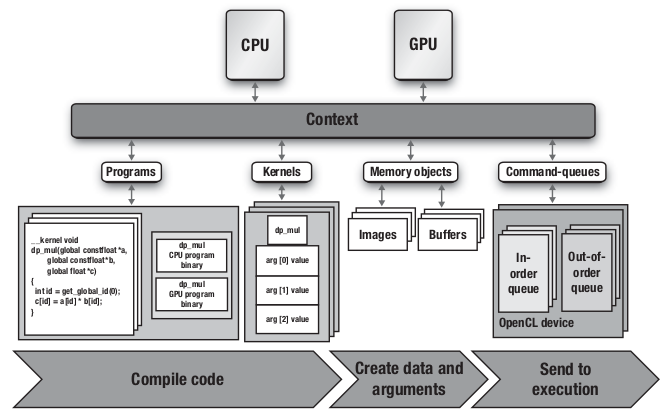
\includegraphics[scale=0.6]{./images/OpenCL_basic_execution_pipeline.png}
  \caption{OpenCL execution pipeline block diagram}
  \label{}
\end{figure}

\begin{enumerate}
	\item We start by defining the context. Here the context contains a CPU and a GPU.
	\item Next we define command-queues. Here we have illustrated two queues viz., in-order and out-of-order queues.
	\item Then the host program defines program objects that are compiled to generate kernels.
	\item The host program then defines memory objets required. This includes memory mapping from kernel arguments to the data memory.
	\item Finally the host program enqueues commands to the command-queues to execute the kernels.
\end{enumerate}

{\color{red} \date{04-June-2020}}
\chapter{HelloWorld with OpenCL}
\section{Adding two arrays}
In this section we are going to learn how to add two arrays in OpenCL. Take a look at the listing below.

\begin{mdframed}[roundcorner=10pt, backgroundcolor=backgroundgray, outerlinewidth=2]
\begin{lstlisting}[frame=none]

#include <iostream>
#include <fstream>
#include <sstream>
#include <CL/cl.h>
#include <string.h>

const int ARRAY_SIZE = 10000;

char* get_program_from_file(const char* file_path)
{
	std::ifstream f(file_path);

	// read all the contents of that file
	std::stringstream f_stream;
	f_stream << f.rdbuf();

	// copy the data to a memory in the heap so that after the scope of this function runs out it still remains
	char* code = (char *)malloc(f_stream.str().length()+1);
	memcpy(code, f_stream.str().c_str(), f_stream.str().length()+1);

	// lets close the open files
	f.close();

	return code;
}

int main()
{
	/* =======================================================================================================
	1) creating a context
	======================================================================================================= */
	// finding out all the platforms on the computer
	unsigned int platformcount;
	clGetPlatformIDs(5, NULL, &platformcount);
	cl_platform_id *platforms = (cl_platform_id *)malloc(sizeof(cl_platform_id) * platformcount);
	clGetPlatformIDs(platformcount, platforms, NULL);

	// creating the context
	cl_context_properties contextproperties[] = {CL_CONTEXT_PLATFORM, (cl_context_properties)platforms[0], 0};
	cl_context context = clCreateContextFromType(contextproperties, CL_DEVICE_TYPE_GPU, NULL, NULL, NULL);

	/* =======================================================================================================
	2) creating a command queue
	======================================================================================================= */
	// we need to get device id first
	unsigned int deviceCount;
	clGetDeviceIDs(platforms[0], CL_DEVICE_TYPE_ALL, 0, NULL, &deviceCount);
	cl_device_id *devices = (cl_device_id *)malloc(sizeof(cl_device_id) * deviceCount);
	clGetDeviceIDs(platforms[0],  CL_DEVICE_TYPE_ALL, deviceCount, devices, NULL);
	cl_command_queue command_queue = clCreateCommandQueue(context, devices[0], 0, NULL);

	/* =======================================================================================================
	3) creating a kernel from the code; building it during runtime
	======================================================================================================= */
	const char* kernel_code = get_program_from_file("./kernel_files/HelloWorld.cl");
	cl_program program = clCreateProgramWithSource(context, 1, (const char**)&kernel_code, NULL, NULL);
	clBuildProgram(program, 0, NULL, NULL, NULL, NULL); // we have omitted build error checks; we need to do that too
    cl_kernel kernel = clCreateKernel(program, "hello_kernel", NULL);

	/* =======================================================================================================
	4) creating data on the host computer
	======================================================================================================= */
    float result[ARRAY_SIZE];
    float a[ARRAY_SIZE];
    float b[ARRAY_SIZE];
    for(unsigned int i=0; i<ARRAY_SIZE; i++)
    {
        a[i] = (float)i;
        b[i] = (float)(i * 2);
    }

	/* =======================================================================================================
	5) creating memory objects for the kernel to use
	======================================================================================================= */
    cl_mem memObjects[3] = {0, 0, 0};
    memObjects[0] = clCreateBuffer(context, CL_MEM_READ_ONLY|CL_MEM_COPY_HOST_PTR, sizeof(float) * ARRAY_SIZE, a, NULL);
    memObjects[1] = clCreateBuffer(context, CL_MEM_READ_ONLY|CL_MEM_COPY_HOST_PTR, sizeof(float) * ARRAY_SIZE, b, NULL);
    memObjects[2] = clCreateBuffer(context, CL_MEM_READ_WRITE, sizeof(float) * ARRAY_SIZE, NULL, NULL);
	// in the kernel code arguments 0, 1, 2 maps to the first set of arguments there
    clSetKernelArg(kernel, 0, sizeof(cl_mem), &memObjects[0]);
    clSetKernelArg(kernel, 1, sizeof(cl_mem), &memObjects[1]);
    clSetKernelArg(kernel, 2, sizeof(cl_mem), &memObjects[2]);

	/* =======================================================================================================
	6) setting worksize info
	======================================================================================================= */
    size_t globalWorkSize[1] = { ARRAY_SIZE };
    size_t localWorkSize[1] = { 1 };
	
    clock_t start, end; 
    start = clock(); 

	// This is where the computation happens; the enqueue command queues up the command in the command_queue. Later when the previous event is finished, this is executed.
    clEnqueueNDRangeKernel(command_queue, 
						   kernel, 
						   1, 
						   NULL, 
						   globalWorkSize, 
						   localWorkSize, 
						   0, 
						   NULL, 
						   NULL);

    end = clock(); 
	std::cout << "Time taken by program is : " << double(end - start)/(double)(CLOCKS_PER_SEC) << std::endl;

	/* =======================================================================================================
	7) reading the buffer back to the host
	======================================================================================================= */
    clEnqueueReadBuffer(command_queue, 
						memObjects[2], // read from mem object 2
						CL_TRUE, // blocking_read - waits for the read to complete before return
						0, 
						ARRAY_SIZE * sizeof(float), 
						result, // into result
						0, 
						NULL, 
						NULL);


	/* printing the result ================================================================================*/
	for(unsigned int i=0; i<ARRAY_SIZE; i++) 
		std::cout << result[i] << " ";

	std::cout << std::endl;

	return 0;
}

\end{lstlisting}
\end{mdframed} 
\pagebreak
Now lets see how the kernel file is programmed.
\begin{mdframed}[roundcorner=10pt, backgroundcolor=backgroundgray, outerlinewidth=2]
%\begin{minipage}[c]{0.95\textwidth}
\begin{lstlisting}[frame=none]
__kernel void hello_kernel(__global const double *a, 
						   __global const double *b, 
						   __global       double *result)
{
    int gid = get_global_id(0);
    result[gid] = a[gid] + b[gid];
}
\end{lstlisting}
%\end{minipage}
\end{mdframed} 

\end{document} 

 
